\chapter{Analysis and specification of needs}
\label{chap:analysis}

\noindent The development process of any application or system requires taking into consideration the needs of the user and their main objectives of using the application.

After researching the current solutions and their drawbacks, we set---within this chapter---to analyze the functional requirements of our users, and therefore our different system actors and their use cases.

\section{Analysis of requirements}

The goal of our project is creating a collaborative visual database that allows users to easily manage their data, be it a list of users, blog posts, or a store inventory, and to easily and securely access this data through an API. Our application is targeted at enterprises and individuals with no or minimal technical skills---a goal that should be kept in mind while structuring our project.

The analysis of requirements phase aims to list a set of both functional and non-functional requirements for modeling and developing our application.

\subsection{Functional requirements}

Functional requirements specify the different tasks of a system. Therefore, in this section, we set the exact tasks that our application must be able to successfully handle, from the most general to the most specific.

\begin{itemize}
	% \tightlist
	\item A user must be able to collaborate with other users on the same document at the same time, in real-time.
	\item A user must be able to organize and share multiple documents at once.
	\item A user must be able to create multiple workspaces.
	\item Each workspace can contain multiple projects containing multiple collections, which in their turn, contain multiple documents.
	\item A user must be able to grant different permissions to different users.
	\item A user must be able to access their documents and collections through an API endpoint.
	\item A user must be able to set a defined structure for their documents.
	\item A user must be able to set predefined filters and queries for each collection, also called a "view".
	\item A user must be able to secure access to their API endpoints.
	\item The API must support real-time updates.
	\item A user must be able to reference other documents.
	\item A user must be able to add rich text to documents.
	\item
	      A user must sign up and login.
	\item
	      A user's account picture must be fetched automatically from Gravatar
	\item
	      A user can upgrade their account to a premium one
	\item
	      A user can cancel their premium subscription
\end{itemize}

\subsection{Non-functional requirements}

Non-functional requirements define \textit{how} a system performs its various tasks. The goal is to offer the best user experience.

\paragraph{Security}

Our application should ensure the security of the hosted data. It should respect the permissions and roles set by the user. Therefore, a robust authentication and authorization system must be put in place.

\paragraph{User experience}

Our goal is to offer the best user experience achievable. Our users will not have must technical knowledge to understand a technically complicated application and they do not have much time to accommodate themselves with a completely new set of interfaces. Our application must be simple and familiar.

\paragraph{Speed}

Our users may not have the best internet connectivity and they might be sharing a single internet connection to accomplish their work. Therefore, our application must load within seconds. This includes caching resources, minifying them, and predicting and preloading what the user is going to need next.

\paragraph{Performance}

Our application has to load and display large amounts of data. This can result in an undesirable glitching and huge memory and CPU usage, which, aside from the slowness of the application, increases the temperature and noise of the computer. Therefore, resulting in an uncomfortable user experience, especially when working within groups.

\paragraph{Accessibility}

Our users might have some preferences when it comes to navigating the interface, such as relying on the keyboard rather than using the cursor. Other users might rely different input devices that require special care. This is an important point to consider in order to render our application usable by as many people as possible.

\paragraph{Scalability}

Our application must be developed with scalability in mind. This includes having to increase the number of servers while maintaining the collaborative aspect of the application.

\paragraph{Developer experience}

Our application must use state-of-the-art technology to offer the best developer experience. This includes using linting and formatting tools, along with deployment platforms such as Docker.

\section{Specification of needs}
\subsection{Identification of actors}

Merebase uses RBAC (Role-Based Access Control) to manage users' access
levels and permissions. There is only one actor, the user, but with
multiple assignable roles.

\begin{itemize}
	% \tightlist
	\item
	      Owner: The user who created the resource, be it the workspace or the
	      project. This role gives you entire access to the resource and it is
	      assigned automatically.
	\item
	      Admin: This role gives non-owner users the same privileges as the
	      owner. Admins can invite new users and assign roles.
	\item
	      Editor: This role permits a user to edit documents in a workspace.
	\item
	      Viewer: This role permits a user to view documents in a workspace,
	      without the ability to modify them.
\end{itemize}

\section{Use case diagrams}

To better illustrate the main interactions between the user and the
application, we rely on a use case diagram.


%\begin{figure}
%\centering
%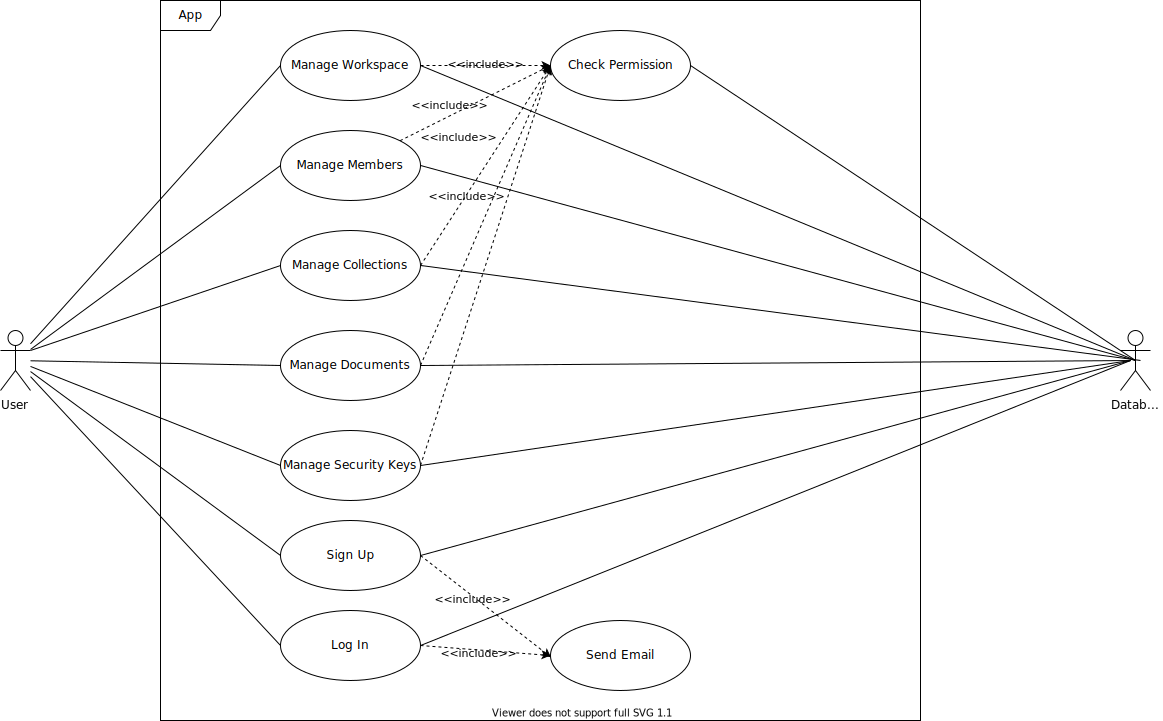
\includegraphics{./assets/UCD, General.svg}
%\caption{General use case diagram}
%\end{figure}

% \begin{tikzpicture}
% 	\draw (0,0) -- (0,4);
% 	\draw (2,2) circle (2);
% \end{tikzpicture}
\begin{figure}[h]
	\centerfloat
	\begin{tikzpicture}

		\begin{umlsystem}[x=4]{Application}
			\umlusecase{use case 1} % usecase-1
			\umlusecase[y=-2]{use case 2} % usecase-2
			\umlusecase[y=-4]{use case 3} % usecase-3
			\umlusecase[x=4, y=-2, width=1.5cm]{ % usecase-4
				\shortstack{use case 4\\\footnotesize{on 2 lines}}
			}
			\umlusecase[x=6, fill=green!20]{use case 5} % usecase-5
			\umlusecase[x=6, y=-4]{use case 6} % usecase-6
		\end{umlsystem}

		\umlactor{user}
		\umlactor[y=-3]{subuser}
		\umlactor[y=-6]{subsubuser}
		\umlactor[x=14, y=-1.5]{admin}

		\umlinherit{subuser}{user}
		\umlinherit{subsubuser}{subuser}
		\umlassoc{user}{usecase-1}
		\umlassoc{subuser}{usecase-2}
		\umlassoc{subuser}{usecase-3}
		\umlassoc{admin}{usecase-5}
		\umlassoc{admin}{usecase-6}
		\umlinherit{usecase-2}{usecase-1}
		\umlVHextend{usecase-5}{usecase-4}
		\umlinclude[name=incl]{usecase-3}{usecase-4}

		% \umlnote[x=7, y=-7]{incl-1}{
		% 		\footnotesize{note on include dependency}
		% }

	\end{tikzpicture}

	\caption{Example of a parametric plot ($\sin (x), \cos(x), x$)}

\end{figure}


\section{Conclusion}

\emph{TBD}